\DiaryEntry{Maximum Flow, Definitions and Basics}{2020-05-27}{Algorithms}

\subsection{Definitions}

A flow network $G = (V,E)$ is a directed graph in which each edge $(u,v) \in E$ has a non-negative capacity $c(u,v) \geq 0$ assigned to it. There is the restriction that if there is an edge $(u,v)$, there is no edge $(v,u)$ in the reverse direction. There are two special vertices in the graph; a source vertex $s$ and a sink vertex $t$.

With this in place, we can formally define flows more formally. A flow in $G$ is a real-valued function $V \times V \rightarrow \mR$ that satisfies the following two properties:

\begin{description}
\item [Capacity Constraint:] The flow along each edge has to be lower than the edge capacity. That is, for all $u,v \in V$, we require $0 \leq f(u,v) \leq c(u,v)$.
\item [Flow Consideration:] For all vertices but $s$ and $t$, the sum of all incoming flows is equal the sum of all outgoing flows. In other words, no flow is or created at the vertices. Formally, we have that fFor all $u \in V - \{s,t\}$, we require

\bee
\sum_{v \in V} f(v,u) = \sum_{v \in V} f(u,v)
\eee

\end{description}

We also define the value $|f|$ of a flow as

\bee
|f| = \sum_{v \in V} f(s,v) - \sum_{v \in V} f(v,s)
\eee

In the maximum-flow probem, we are given a flow network with a source vertex $s$ and sink $t$, and we want to find a flow of maximum value.

\paragraph{Example.} The following Figure shows an example flow network. The labels of the edges follow the convention $f(u,v)/c(u,v)$. So for example, the capacity on the edge $(2,1)$ is $4$, the actual flow along this egde is $1$. 

\begin{figure}[H]
\centering
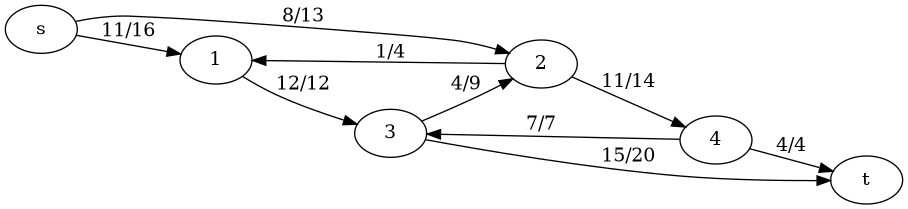
\includegraphics[scale=0.5]{images/max_flow_01.png}
\end{figure}


\subsection{TODO}

Antiparallel edges

multiple sources and sinks

\subsection{Ford-Fulkerson Method}

The Ford-Fulkerson Method solves the maxium-flow problem. It is a method and not an algoritmh, as it provides several implementation options. Ford-Fulkeron is based on three ideas: Residual networks, augmenting paths, and cuts.

The method iteratively increases the value of the flow. We start with $f(u,v)=0$ for all $u,v \in V$, giving an initial flow of value of $0$. At each iteration, we increase the flow value by finding an ``augmenting'' path in an associated ``residual network'' $G_f$.

Once we know the edges of an augmenting path in $G_f$ , we can easily identify specific edges in $G$ for which we can change the flow so that we increase the value of the flow. Although each iteration of the Ford-Fulkerson method increases the value of the flow, we shall see that the flow on any particular edge of $G$ may increase or decrease; decreasing the flow on some edges may be necessary in order to enable an algorithm to send more flow from the source to the sink. We repeatedly augment the flow until the residual network has no more augmenting paths. The max-flow min-cut theorem will show that upon termination, this process yields a maximum flow.

The Ford-Fulkerson Method looks as follows

\begin{Verbatim}[numbers=left, xleftmargin=5mm]
Ford-Fulkerson(G,s,t)
   initialize flow f to 0
   while there exists an augmenting path p in the residula network G_f
      augment flow f along p
   return f
\end{Verbatim}


\subsubsection{Residual Networks}

\subsubsection{Augmenting Paths}

\subsubsection{Cuts of FLow Networks}

\subsection{Basic Ford-Fulkerson Algorithm}




%%% Local Variables:
%%% mode: latex
%%% TeX-master: "journal"
%%% End:
